\begin{figure}[p]
    \centering
    \begin{minipage}[b]{.48\textwidth}
        \begin{figure}[H]
            \centering
            \subfigure[determinant of the symmetric part of the elastoplastic modulus tensor 弹塑性模量张量的对称部分的行列式的演变]{
                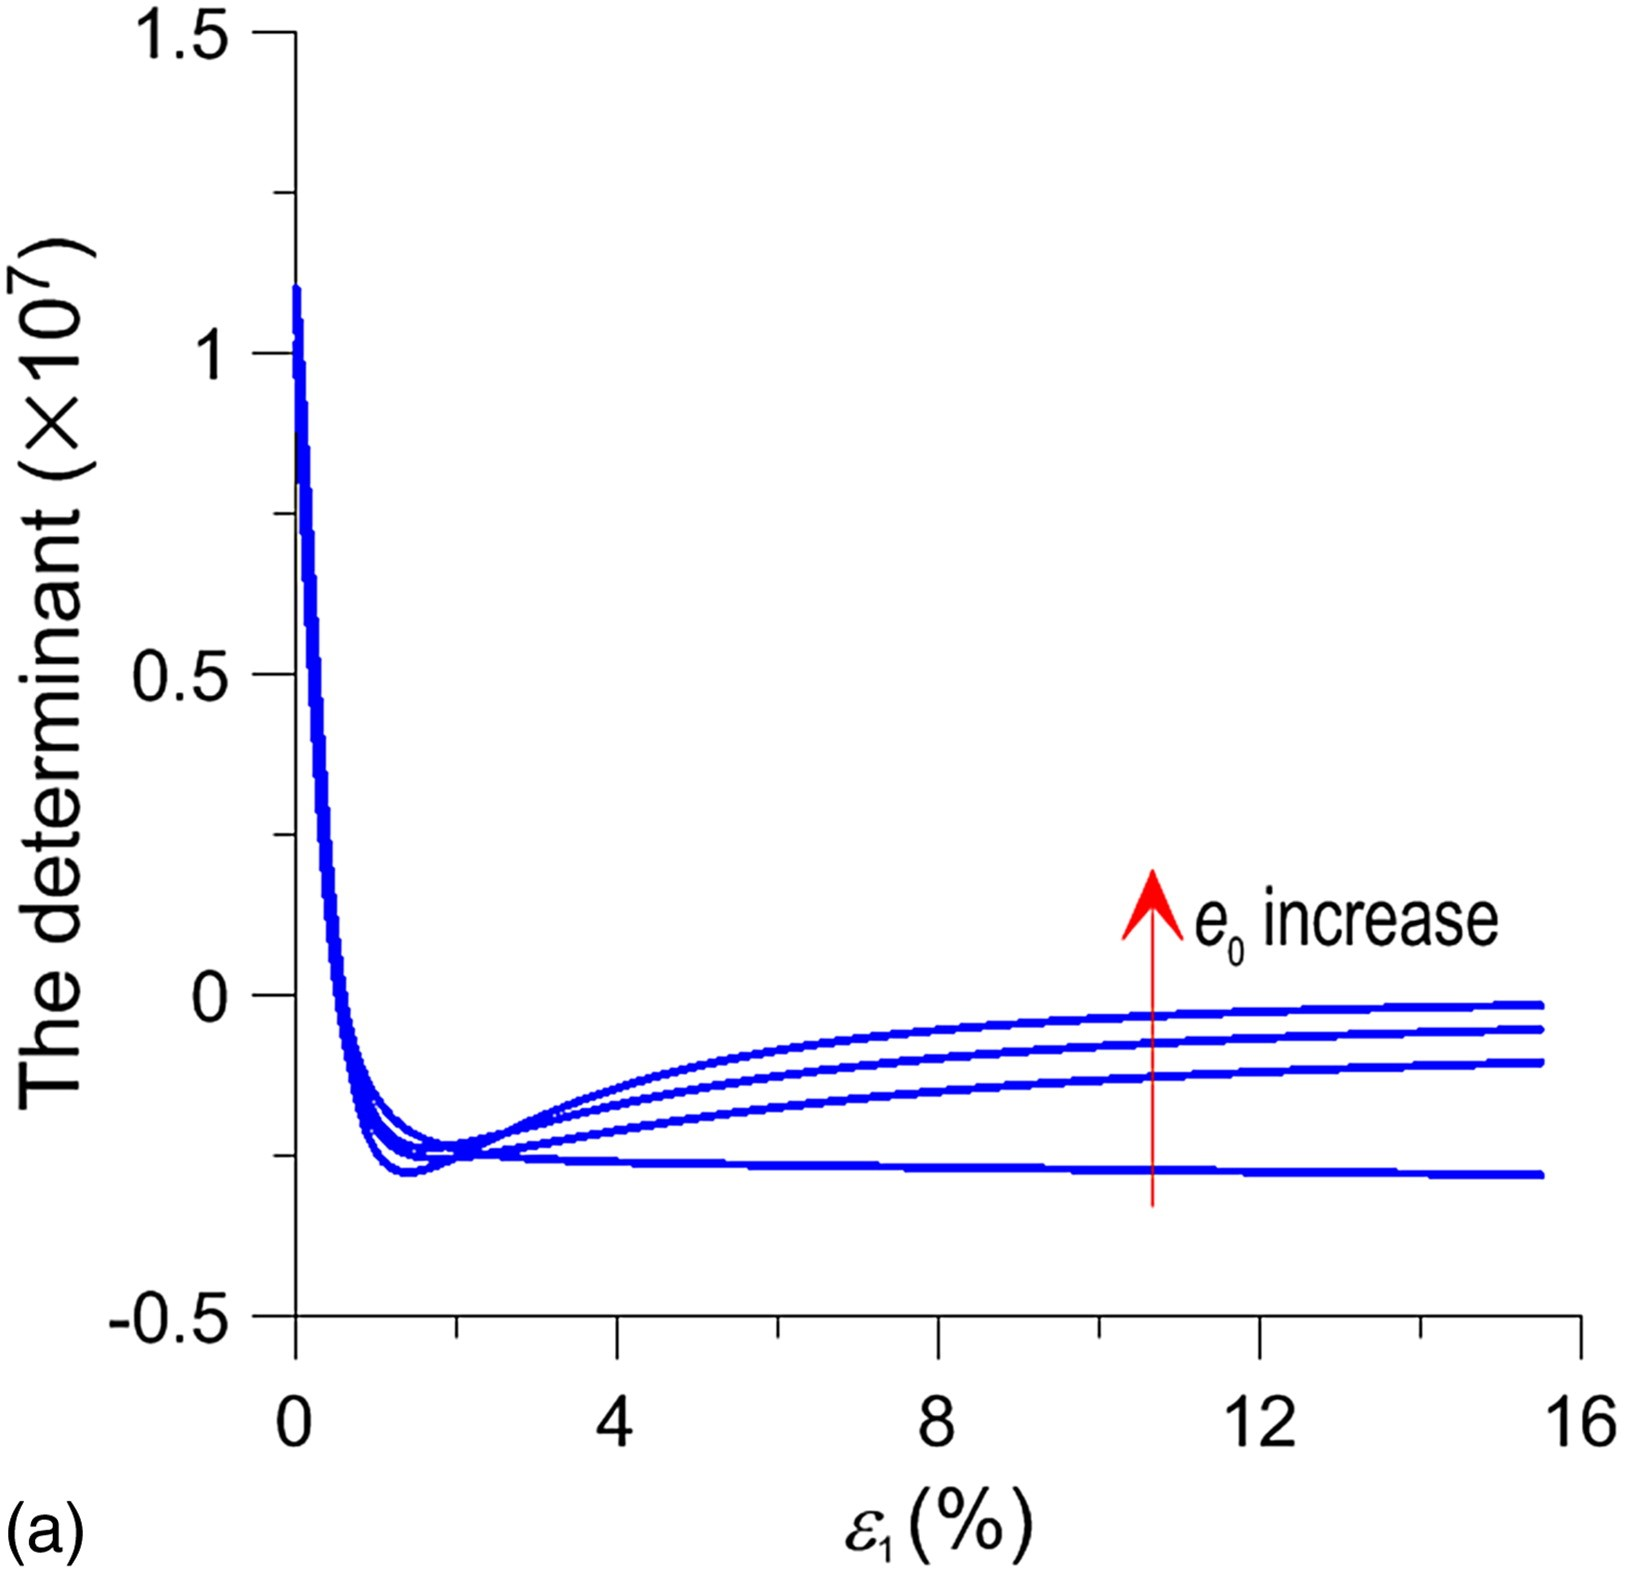
\includegraphics[width=\textwidth]{figures/figure11a.jpg}
                \label{figure:11a}
            }
            \subfigure[evolution of second-order work 二阶功]{
                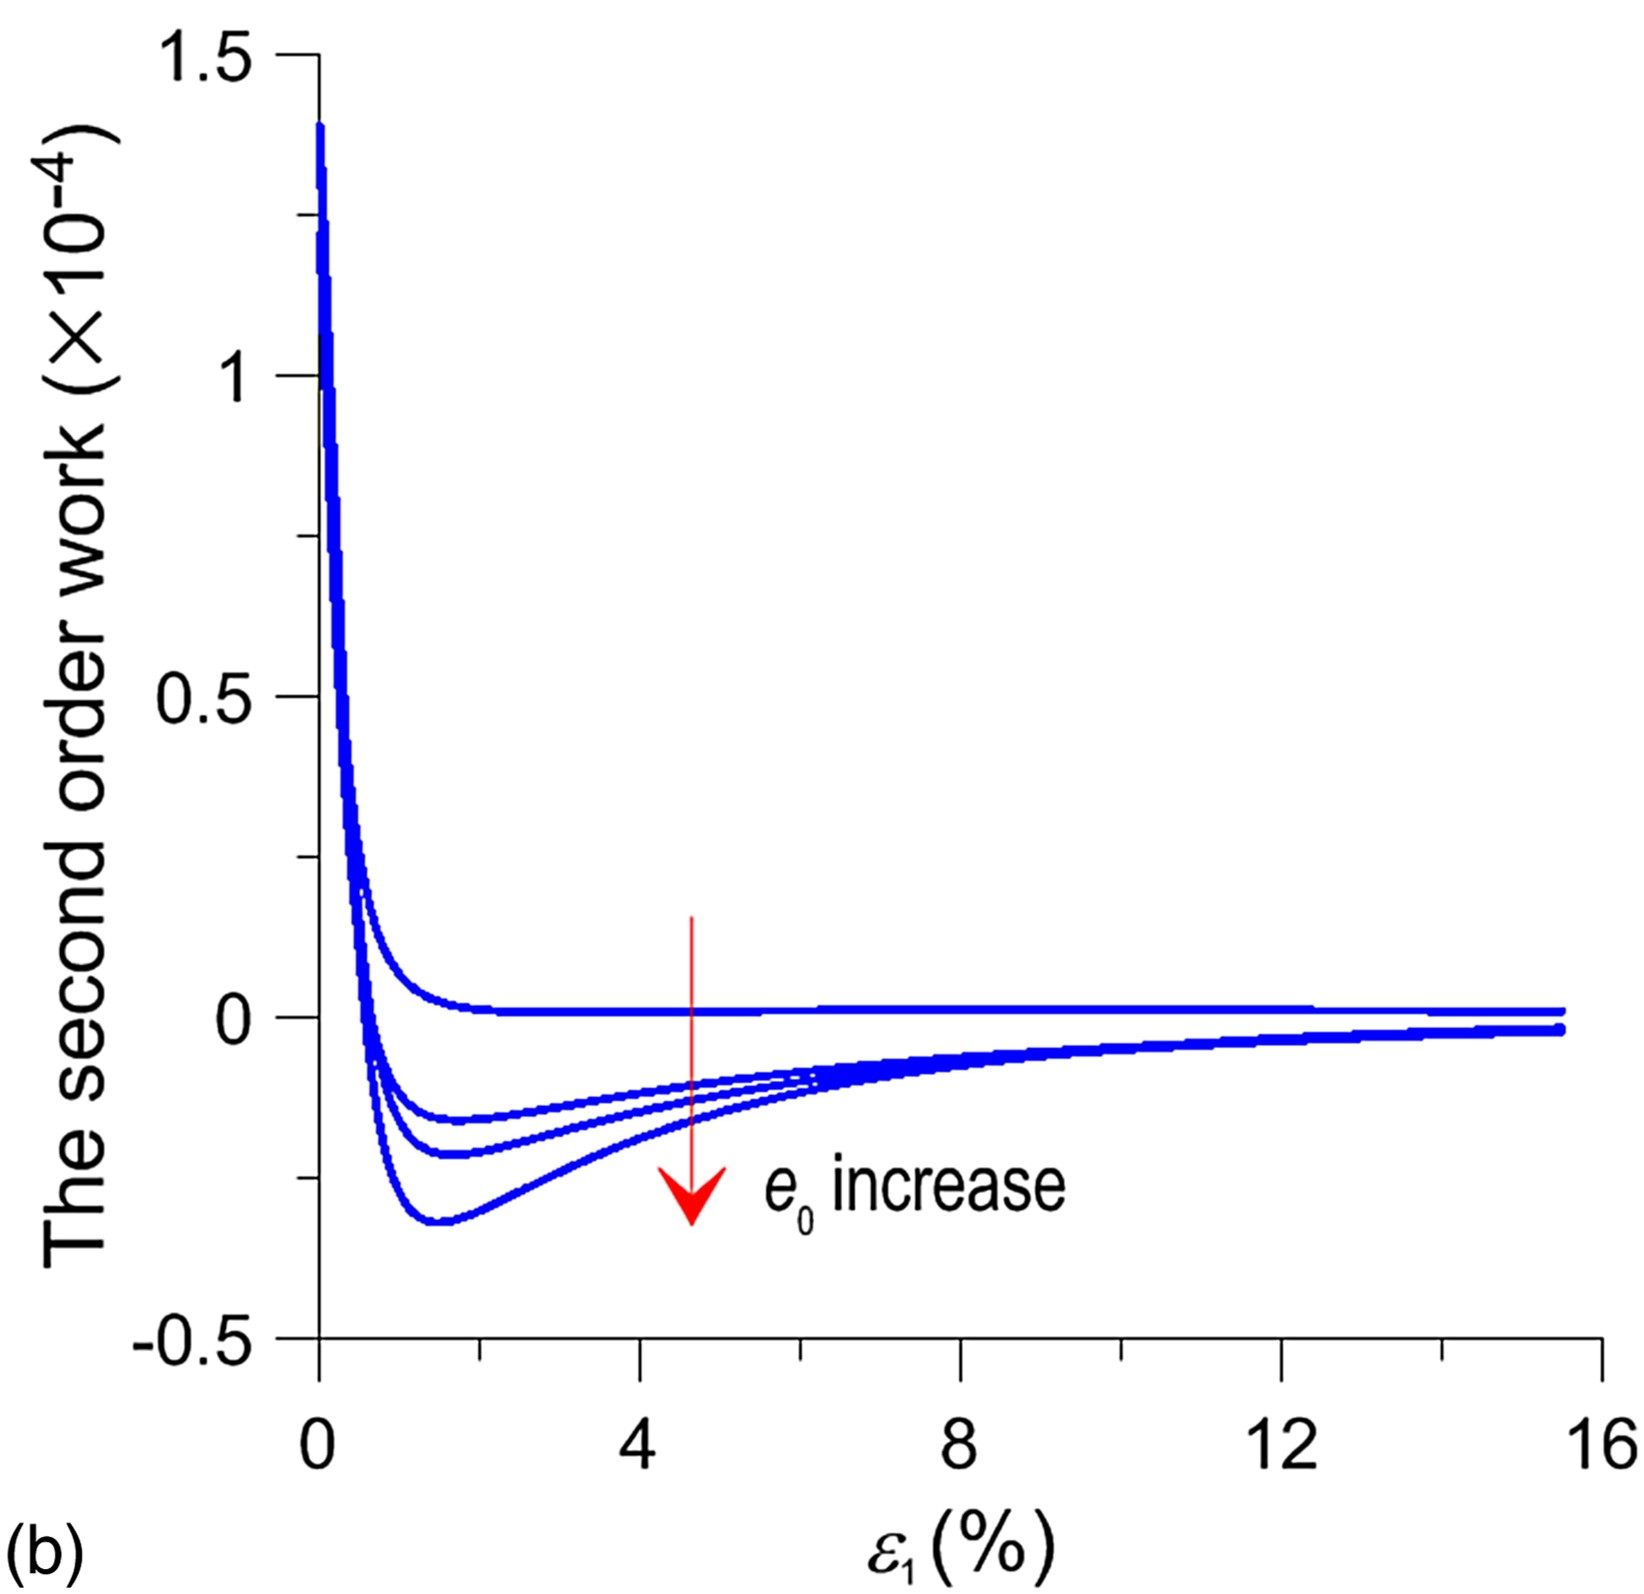
\includegraphics[width=\textwidth]{figures/figure11b.jpg}
                \label{figure:11b}
            }
            \bicaption{Evolution of determinant of the symmetric part of the elastoplastic modulus tensor and second-order work}{弹塑性模量张量的对称部分的行列式的和二阶功的演变}
            \label{figure:11}
        \end{figure}
    \end{minipage}
    \hspace{0.02\textwidth}
    \begin{minipage}[b]{.48\textwidth}
        \begin{figure}[H]
            \centering
            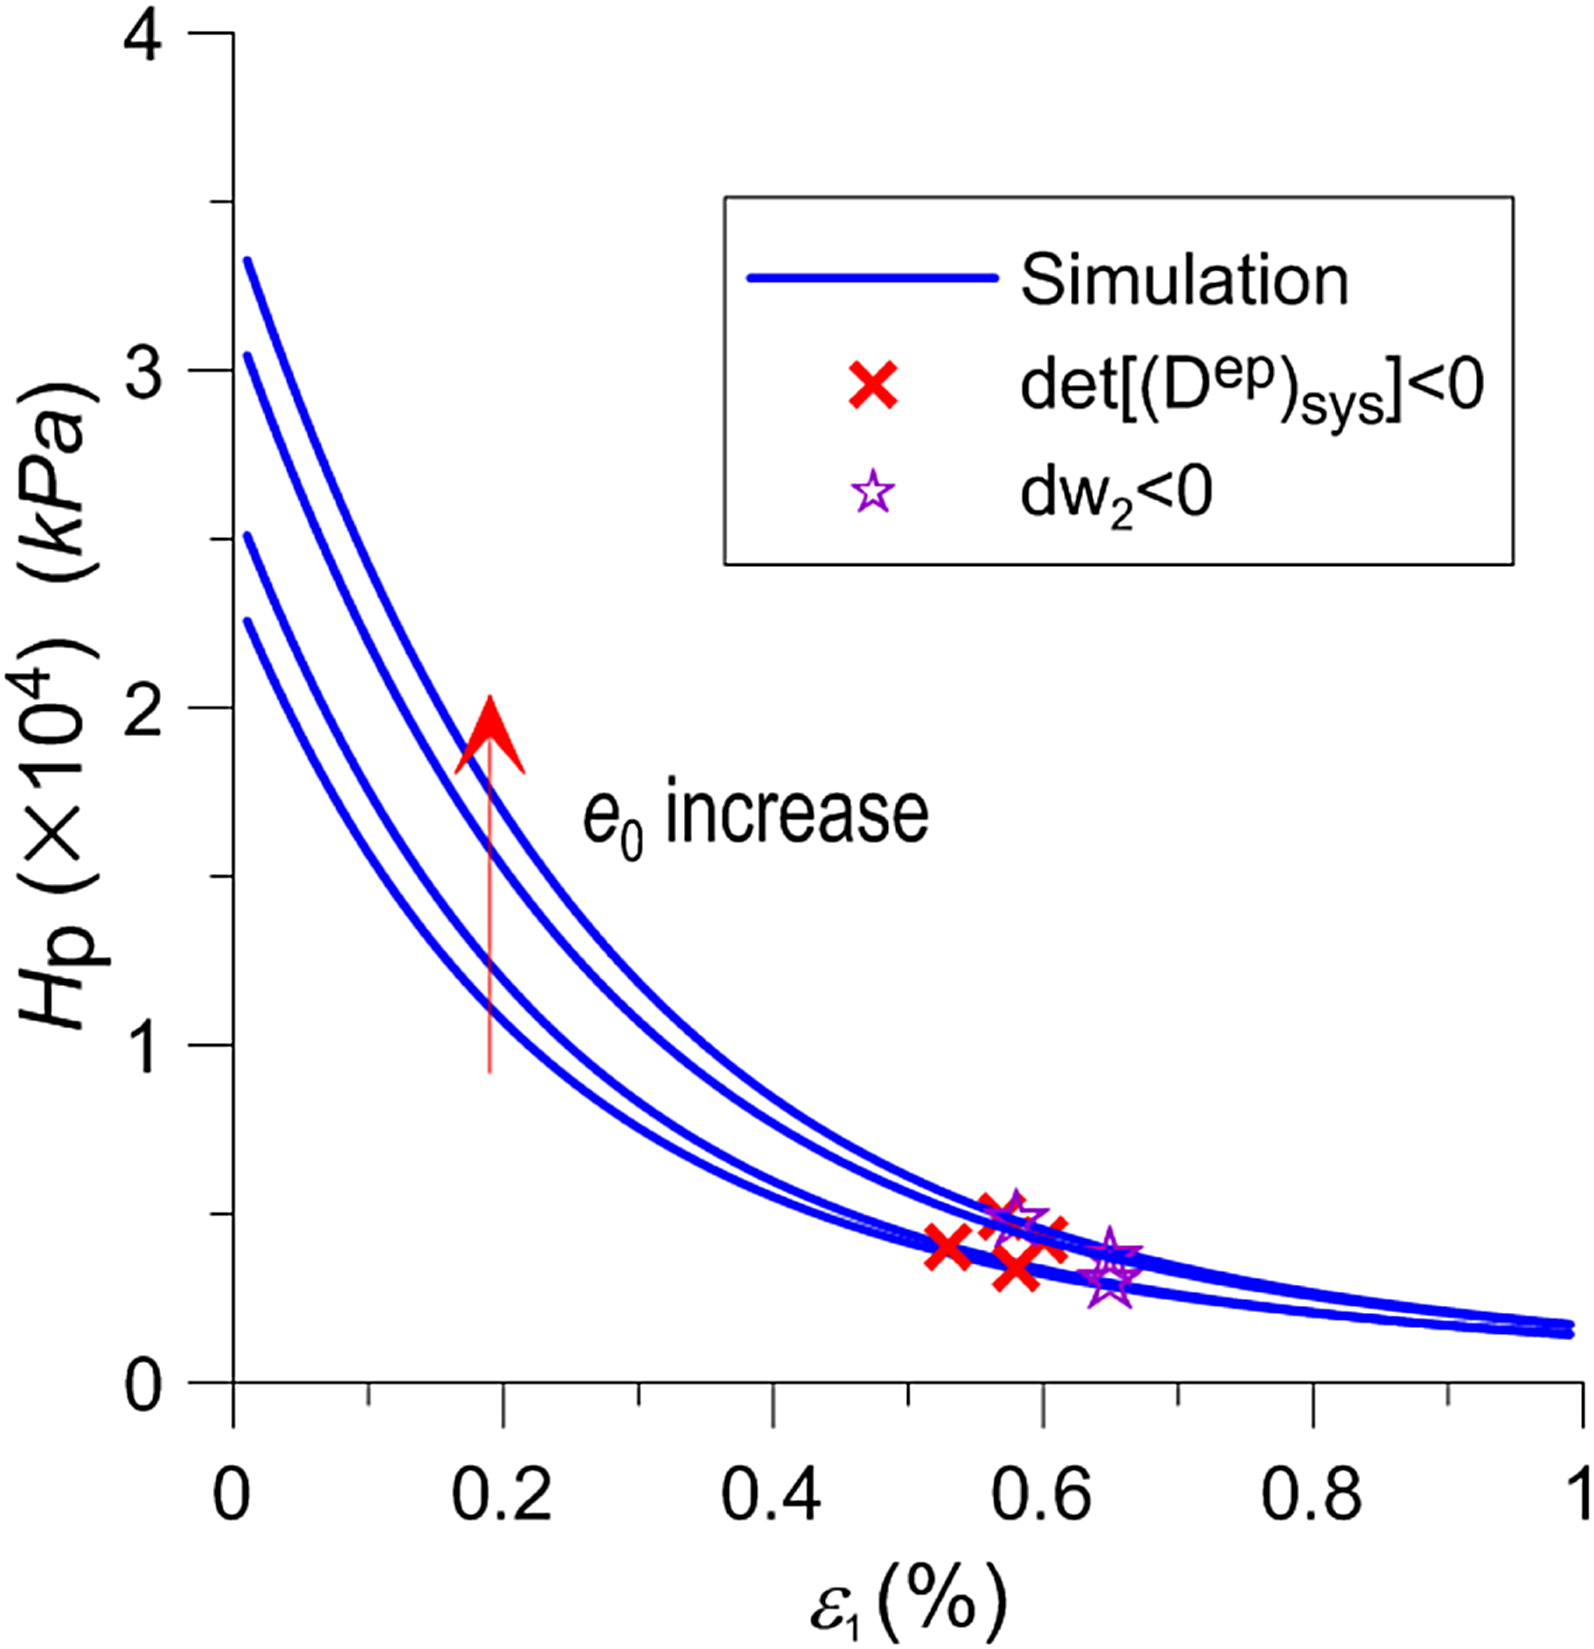
\includegraphics[width=\textwidth]{figures/figure12.jpg}
            \bicaption{Evolution of hardening modulus}{硬化模量的演变}
            \label{figure:12}
        \end{figure}
        \begin{figure}[H]
            \centering
            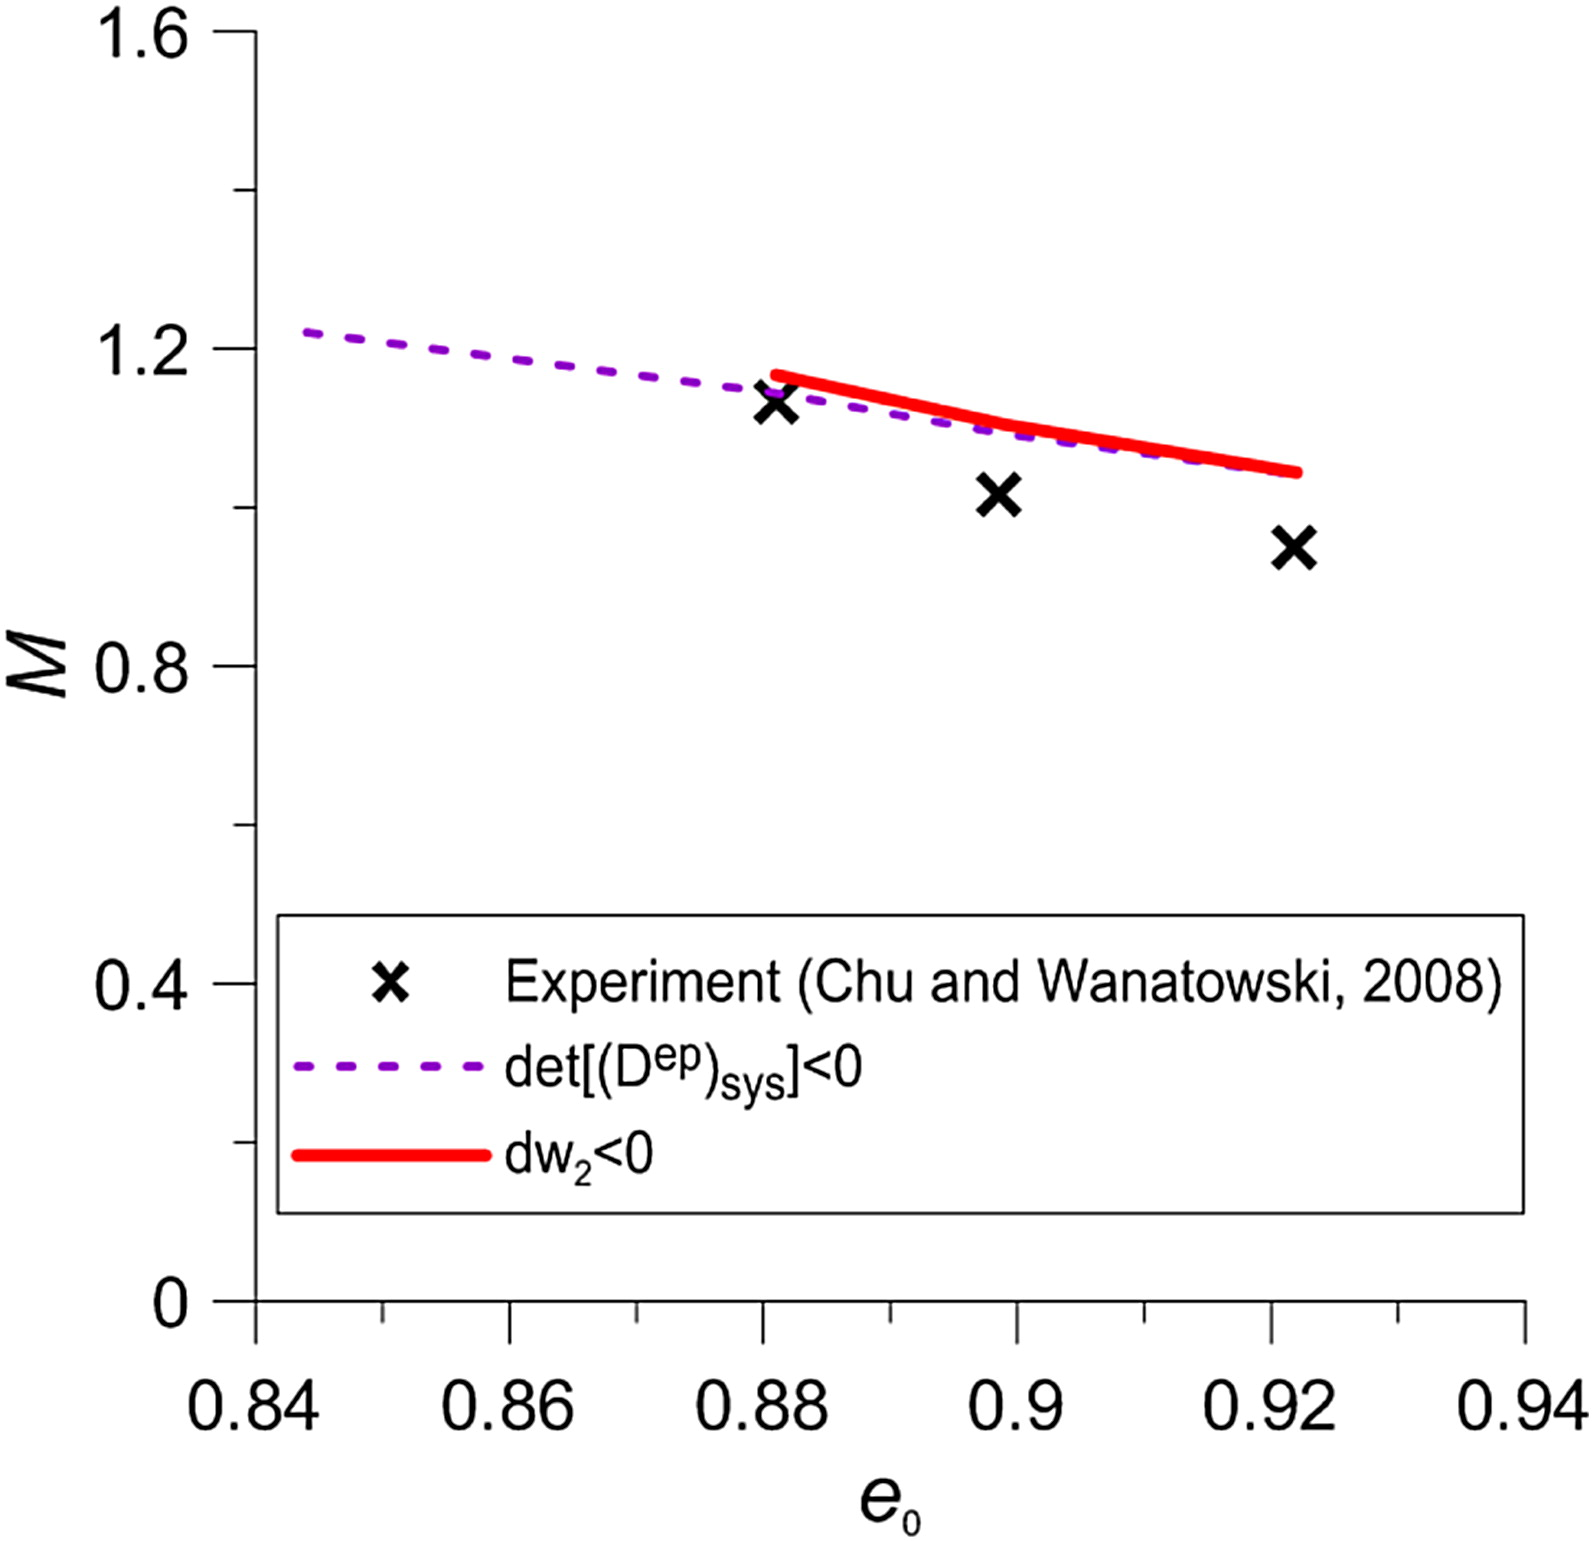
\includegraphics[width=\textwidth]{figures/figure13.jpg}
            \bicaption{Influence of the initial void ratio on the stress ratio at the onset of static liquefaction}{初始液化比对静态液化开始时应力比的影响}
            \label{figure:13}
        \end{figure}
    \end{minipage}
\end{figure}